\documentclass[11pt]{article}
\usepackage{amssymb}
\usepackage{amsthm}
\usepackage{enumitem}
\usepackage{physics,amsmath}
\usepackage{bm}
\usepackage{adjustbox}
\usepackage{mathrsfs}
\usepackage{graphicx}
\usepackage{siunitx}
\usepackage[mathscr]{euscript}

\title{\textbf{Solved selected problems of Classical Mechanics - Gregory}}
\author{Franco Zacco}
\date{}

\addtolength{\topmargin}{-3cm}
\addtolength{\textheight}{3cm}

\newcommand{\hatr}{\bm{\hat{r}}}
\newcommand{\hatx}{\bm{\hat{x}}}
\newcommand{\haty}{\bm{\hat{y}}}
\newcommand{\hatz}{\bm{\hat{z}}}
\newcommand{\hatth}{\bm{\hat{\theta}}}
\newcommand{\hatphi}{\bm{\hat{\phi}}}
\newcommand{\hatrho}{\bm{\hat{\rho}}}
\theoremstyle{definition}
\newtheorem*{solution*}{Solution}
\renewcommand*{\proofname}{\bf{Solution}}

\begin{document}
\maketitle
\thispagestyle{empty}

\section*{Chapter 11 - The angular momentum principle}

	\begin{proof}{\textbf{11.3}}
    The system described looks like the following
    \begin{center}
        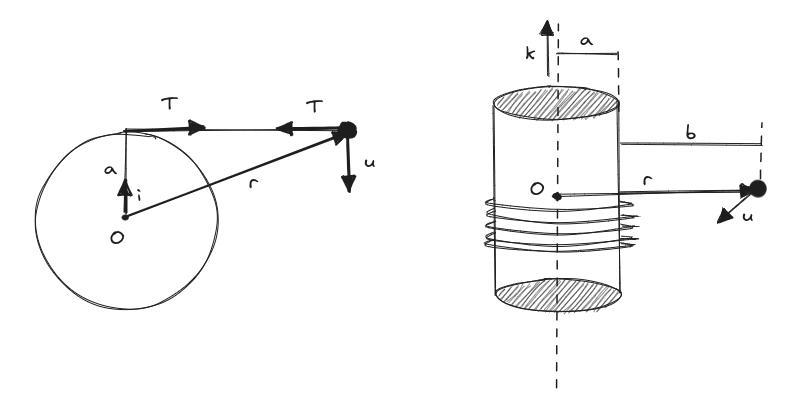
\includegraphics[scale=0.55]{ch11-3.png}
    \end{center}
    From the diagram, the total moment of the external forces about $O$ is
    \begin{align*}
        \bm{K_O} = [(a\bm{i}) \times \bm{T}] - [(a\bm{i}) \times \bm{T}]
        + [\bm{0} \times -Mg\bm{k}] + [\bm{r} \times -mg\bm{k}]
    \end{align*}
    So we see that $\bm{K_O} \cdot \bm{k} = 0$ since the tensions on the string
    are opposite and the gravitational component of the particle gives us
    $-mg\bm{r} \cdot (\bm{k} \times \bm{k}) = 0$. Hence $\bm{L_O} \cdot \bm{k}$
    the angular momentum of the system about the rotation axis is conserved.

    It follows that this axial angular momentum is the same at the beginning
    and the end of the movement.
    Initially, the cylinder is at rest and the particle has a velocity $\bm{u}$
    perpendicular to the string with length $b$ describing for the first
    instant a circular orbit with radius $b$ then
    \begin{align*}
        \bm{L_O} \cdot \bm{k} &= mbu
    \end{align*}
    And when the particle finally sticks to the cylinder we get that
    \begin{align*}
        \bm{L_O} \cdot \bm{k} = \bigg(\frac{1}{2}Ma^2\bigg)\Omega +  ma^2\Omega
    \end{align*}
    Since $\bm{L_O} \cdot \bm{k}$ is known to be conserved it follows that
    \begin{align*}
        \bigg(\frac{1}{2}Ma^2\bigg)\Omega +  ma^2\Omega &= mbu\\
        \Omega\bigg(\frac{a^2}{2}(M + 2m)\bigg) &= mbu\\
        \Omega &= \frac{2mbu}{a^2(M+2m)}
    \end{align*}
    \end{proof}
\begin{proof}{\textbf{11.4}}
        Let $\bm{k}$ be a unit vector in the direction of the rotational axis
        through the center of the gas sphere. Given that the cloud can move
        freely in space and there are no forces applied to it we have that
        $$\bm{K_0}\cdot\bm{k} = 0$$
        Hence $\bm{L_O} \cdot \bm{k}$ the angular momentum of the system about
        the rotation axis is conserved.

        It follows that this axial angular momentum is the same at the
        beginning and the end of the movement. Initially, the cloud has the
        form of a uniform sphere then
        \begin{align*}
            \bm{L_O} \cdot \bm{k} = \bigg(\frac{2}{5}Ma^2\bigg)\Omega
        \end{align*}
        Then the cloud has the form of a thin uniform circular disk hence
        \begin{align*}
            \bm{L_O} \cdot \bm{k} = \bigg(\frac{1}{2}Mb^2\bigg)\Omega'
        \end{align*}
        Since $\bm{L_O} \cdot \bm{k}$ is known to be conserved it follows that
        \begin{align*}
            \bigg(\frac{1}{2}Mb^2\bigg)\Omega' &= \bigg(\frac{2}{5}Ma^2\bigg)\Omega\\
            \Omega' &= \frac{4}{5}\frac{a^2}{b^2} \Omega
        \end{align*}
        Finally, the initial and final kinetic energies of the system are
        \begin{align*}
            \frac{1}{2}\bigg(\frac{2}{5}Ma^2\bigg)\Omega^2
            \quad\text{and}\quad
            \frac{1}{2}\bigg(\frac{1}{2}Mb^2\bigg)\Omega'^2
        \end{align*}
        On using the value of $\Omega'$ found above and simplifying,
        the kinetic energy of the system is found to increase by
        \begin{align*}
            \Delta T &=
            \frac{1}{2}\bigg(\frac{1}{2}Mb^2\bigg)
            \bigg(\frac{4}{5}\frac{a^2}{b^2} \Omega\bigg)^2
            - \frac{1}{2}\bigg(\frac{2}{5}Ma^2\bigg)\Omega^2\\
            &= \frac{4Ma^4}{25b^2}\Omega^2 - \frac{1}{5}Ma^2\Omega^2\\
            &= \frac{Ma^2}{25b^2}(4a^2 - 5b^2)\Omega^2
        \end{align*}
\end{proof}
\cleardoublepage
\begin{proof}{\textbf{11.5}}
    The system described in the two stages looks like the following
    \begin{center}
        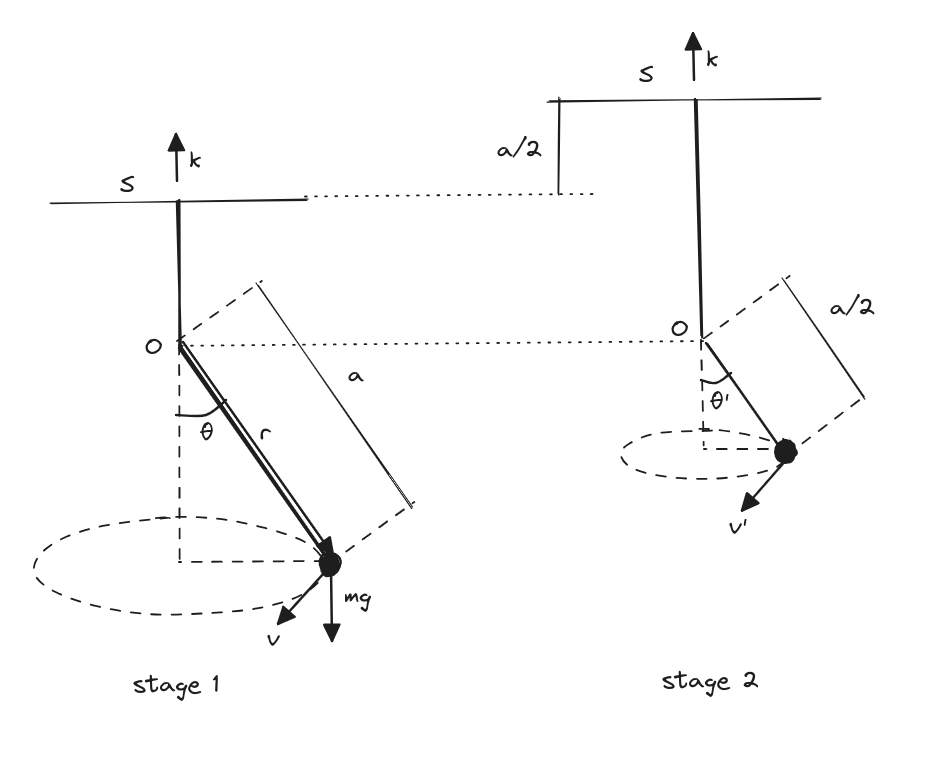
\includegraphics[scale=0.48]{ch11-5.png}
    \end{center}
    Let's first analyze Newton's equation of the conical pendulum shown
    \begin{align*}
        T\cos\theta - mg = 0\\
        T\sin\theta = \frac{mv^2}{a\sin \theta}
    \end{align*}
    Where we take into account the components of the string tension and the 
    centripetal acceleration. Hence the tangential velocity $v$ of the particle
    is given by
    \begin{align*}
        \frac{g \sin\theta}{\cos\theta} = \frac{v^2}{a\sin \theta}\\
        v = \sqrt{\frac{ga}{\cos\theta}} \sin\theta
    \end{align*} 
    Let's analyze the moment with respect to $O$. From the diagram, the
    total moment of the external forces about $O$ is
    \begin{align*}
        \bm{K_O} = (\bm{0} \times \bm{T}) + (\bm{r} \times \bm{T})
        + (\bm{r} \times -Mg\bm{k})
    \end{align*}
    So we see that $\bm{K_O} \cdot \bm{k} = 0$ since
    $\bm{0} \times \bm{T} = \bm{0}$, also $\bm{r} \times \bm{T} = \bm{0}$
    since they are parallel vectors.
    The gravitational component of the particle gives us
    $-mg\bm{r} \cdot (\bm{k} \times \bm{k}) = 0$. Hence $\bm{L_O} \cdot \bm{k}$
    the angular momentum of the system about the rotation axis is conserved.
    
    It follows that this axial angular momentum is the same at the beginning
    and at the end of the movement. Initially, the particle is rotating on a 
    circular path of radius $a \sin \theta$ with an tangential velocity we
    derived above then
    \begin{align*}
        \bm{L_0 \cdot k} &= m \cdot \sqrt{\frac{ga}{\cos\theta}} \sin\theta
            \cdot a \sin \theta\\
            &= ma \sqrt{\frac{ga}{\cos\theta}} \sin^2\theta
    \end{align*}
    In stage 2, where the string has reduced to a length of $a/2$ we have that
    \begin{align*}
        \bm{L_0 \cdot k} &= m \cdot \sqrt{\frac{ga}{2\cos\theta'}} \sin\theta'
        \cdot \frac{a \sin \theta'}{2}\\
        &= \frac{ma}{2} \sqrt{\frac{ga}{2\cos\theta'}} \sin^2\theta'
    \end{align*}
    Since $\bm{L_O} \cdot \bm{k}$ is known to be conserved it follows that
    \begin{align*}
        \frac{ma}{2} \sqrt{\frac{ga}{2\cos\theta'}} \sin^2\theta'
        &= ma \sqrt{\frac{ga}{\cos\theta}} \sin^2\theta\\
        \frac{ga}{8\cos\theta'} \sin^4\theta'
        &=\frac{ga}{\cos\theta} \sin^4\theta\\
        \frac{\sin^4\theta'}{\cos\theta'} &= 9
    \end{align*}
    Where we used that initial angle is $\theta = 60^\circ$. Finally, by
    solving the equation numerically we find that $\theta' = 83.77^\circ$.
\end{proof}
\cleardoublepage
\begin{proof}{\textbf{11.7}}
    Let's consider the system described below 
    \begin{center}
        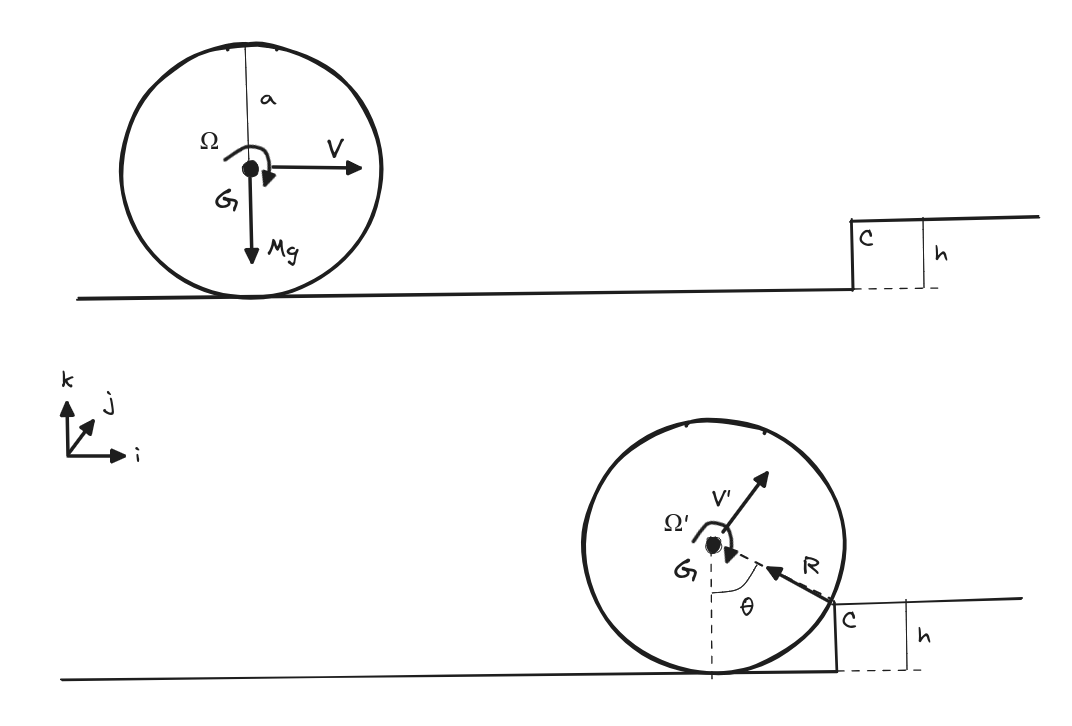
\includegraphics[scale=0.40]{ch11-7.png}
    \end{center}
    From the diagram, initially, the momentum around $C$ is given by 
    \begin{align*}
        \bm{L_C} &= M(a-h)V\bm{j} + Ma^2 \Omega\bm{j}\\
            &= M(2a-h)V\bm{j}
    \end{align*}
    where $I = Ma^2$ is the moment of inertia of the hoop with respect to $G$
    and since we assume the movement is a rotation without slipping the
    tangential velocity is also $V = a\Omega$.

    Let's analyze now the moment right after the hoop encounters the step, then
    we have that
    \begin{align*}
        \bm{L_C} &= MaV'\bm{j} + Ma^2 \Omega'\bm{j}\\
            &= 2MaV'\bm{j}
    \end{align*}
    Since the momentum is known to be conserved we get that the instantaneous
    speed of the center of mass is
    \begin{align*}
        2MaV' &= M(2a-h)V\\
        V' &= \bigg(1 - \frac{h}{2a}\bigg)V 
    \end{align*}
    and the instantaneous angular velocity of the hoop is
    \begin{align*}
        \Omega' &= \bigg(1 - \frac{h}{2a}\bigg)\frac{V}{a} 
    \end{align*}
\cleardoublepage
    Now that the hoop is at the step, there are two options either the hoop
    goes up the step where the center of mass performs an arc trajectory and
    the particle $C$ remains in contact with the step (at rest) or the particle
    $C$ does not remain in contact with the step. 
    Let's now decompose the forces in the $GC$ direction assuming the particle
    $C$ remains in contact with the step
    \begin{align*}
        \frac{MV'^2}{a} &= Mg\cos\theta - R\\
        R &= Mg\frac{a-h}{a} - \frac{M}{a}\bigg(1 - \frac{h}{2a}\bigg)^2V^2
    \end{align*}
    where we used that $\cos\theta = (a-h)/a$ and we replaced the value we got
    for $V'$. If $Mg\cos\theta < R$ then the particle $C$ will not stay in
    contact with the step and this will happen if
    \begin{align*}
        \frac{M}{a}\bigg(1 - \frac{h}{2a}\bigg)^2V^2 &> Mg\frac{(a-h)}{a}\\
        V^2 &> g(a-h) \bigg(1 - \frac{h}{2a}\bigg)^{-2}
    \end{align*}
    Suppose now that the particle $C$ does remain on the edge of the step.
    Then for the hoop to mount the step is necessary some energy to raise
    it there, by applying the conservation of energy we have that
    \begin{align*}
        \frac{1}{2}MV'^2 + \frac{1}{2}(Ma^2)\bigg(\frac{V'}{a}\bigg)^2 + Mga
        &>  Mg(a+h)\\
        V'^2 + ga &>  g(a+h)\\
        V^2 &> gh\bigg(1 - \frac{h}{2a}\bigg)^{-2} 
    \end{align*}
    If we want the hoop to stay still in contact with the step and to mount it
    we need both the following conditions at the same time
    \begin{align*}
        V^2 &< g(a-h) \bigg(1 - \frac{h}{2a}\bigg)^{-2}
    \end{align*}
    and that
    \begin{align*}
        V^2 &> gh\bigg(1 - \frac{h}{2a}\bigg)^{-2}
    \end{align*}
    This implies that
    \begin{align*}
        gh\bigg(1 - \frac{h}{2a}\bigg)^{-2}
        &< g(a-h) \bigg(1 - \frac{h}{2a}\bigg)^{-2}\\
        h &< a/2 
    \end{align*}
    Therefore if the step is higher than $a/2$ the hoop cannot mount the step
    and stay in touch with it.
\end{proof}
\cleardoublepage
\begin{proof}{\textbf{11.8}}
    Let's consider the system described below
    \begin{center}
        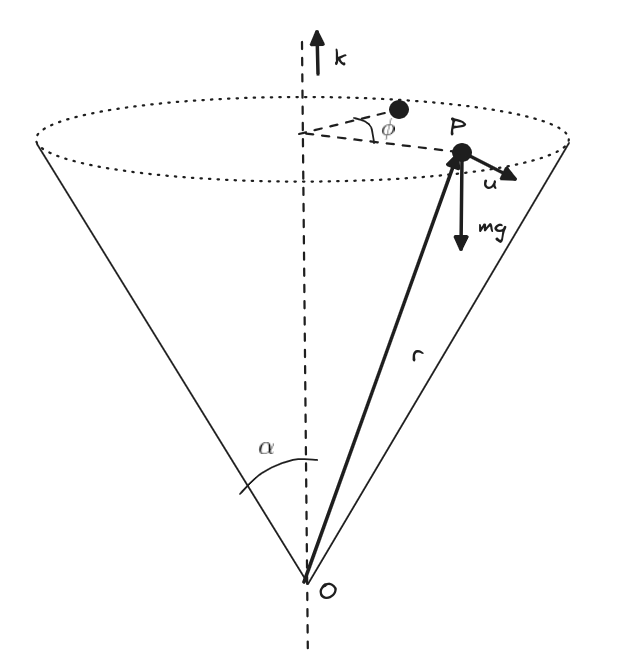
\includegraphics[scale=0.40]{ch11-8.png}
    \end{center}
    Let's analyze the moment with respect to the vertical axis through $O$.
    From the diagram, the total moment of the external forces about $O$ is
    \begin{align*}
        \bm{K_O} = \bm{r} \times -mg\bm{k} + \bm{r} \times \bm{N}
    \end{align*}
    So we see that $\bm{K_O} \cdot \bm{k} = 0$ since the gravitational
    component of the particle gives us
    $-mg\bm{r} \cdot (\bm{k} \times \bm{k}) = 0$ and
    $(\bm{r} \times \bm{N}) \cdot \bm{k} = 0$ because the vectors are all in
    the same plane.
    Hence $\bm{L_O} \cdot \bm{k}$ the angular momentum of the system about
    the vertical axis is conserved.
    
    Initially, the particle is a distance $a$ from $O$ and is horizontally
    projected with a velocity $u$ hence
    \begin{align*}
        \bm{L_0 \cdot k} = m (a\sin\alpha) u
    \end{align*}
    Later the momentum in the vertical direction has a tangential velocity
    of $(r \sin\alpha )\dot{\phi}$ where $\dot{\phi}$ is the angular velocity
    in the azimuthal direction then
    \begin{align*}
        \bm{L_0 \cdot k} = m (r \sin\alpha)(r \sin\alpha)\dot{\phi}
    \end{align*}
    And since the momentum in the vertical direction is known to be conserved
    we have that
    \begin{align*}
        m (r \sin\alpha)^2\dot{\phi} &= m (a\sin\alpha) u\\
        r^2 \dot{\phi} \sin\alpha &= au \\
        \dot{\phi} &= \frac{au}{r^2 \sin \alpha}
    \end{align*}
    Also, given that the cone is smooth (hence the constraint force does not
    work) and the gravitational force acting on the particle is a conservative
    force then the energy is conserved. Initially, the particle has an energy
    given by 
    \begin{align*}
        E = \frac{1}{2}m u^2 + mg (a \cos \alpha) 
    \end{align*}
    Later the particle would have an energy of
    \begin{align*}
        E = \frac{1}{2}m \dot{r}^2 + \frac{1}{2}m (r \sin\alpha \dot{\phi})^2 + mg (r \cos \alpha) 
    \end{align*}
    And since we know that energy is conserved we have that
    \begin{align*}
        \frac{1}{2}m \dot{r}^2 + \frac{1}{2}m (r \sin\alpha \dot{\phi})^2 + mg (r \cos \alpha)
        &= \frac{1}{2}m u^2 + mg (a \cos \alpha)\\
        \dot{r}^2 + (r \sin\alpha \dot{\phi})^2 + 2g (r \cos \alpha)
        &= u^2 + 2g(a \cos \alpha)\\
        \dot{r}^2 = u^2 - (r \sin\alpha \dot{\phi})^2 &+ 2g\cos \alpha(a - r)
    \end{align*}
    Now replacing the value we have for $\dot{\phi}$ we get the value for
    $\dot{r}^2$ that we want
    \begin{align*}
        \dot{r}^2 &= u^2 - \frac{a^2u^2}{r^2} + 2g\cos \alpha(a - r)\\
        \dot{r}^2 &= \frac{u^2}{r^2}(r^2 - a^2) + 2g\cos \alpha(a - r)\\
        \dot{r}^2 &= (r - a)\bigg[\frac{u^2}{r^2}(r + a) - 2g\cos \alpha\bigg]
    \end{align*}
    \textbf{Case A.} In the absence of gravity $(g=0)$, we get that $r$
    is given by
    \begin{align*}
        \dot{r}^2 &= \frac{u^2}{r^2}(r^2 - a^2)\\
        \frac{dr}{dt} &= \frac{u}{r}\sqrt{r^2 - a^2}\\
        \int \frac{r}{\sqrt{r^2 - a^2}} dr &= u \int dt\\
        \sqrt{r^2 - a^2} &= ut\\
        r &= \sqrt{(ut)^2 + a^2}
    \end{align*}
    And from the value we have for $\dot{\phi}$ by replacing $r$ we can
    determine $\phi$ as follows
    \begin{align*}
        \frac{d\phi}{dt} &= \frac{au}{((ut)^2 + a^2) \sin \alpha}\\
        \int d\phi &= \frac{au}{\sin \alpha} \int \frac{dt}{(ut)^2 + a^2}\\
        \phi &= \frac{au}{\sin \alpha} \frac{\arctan(ut/a)}{au}\\
        \phi &= \frac{\arctan(tu/a)}{\sin \alpha}
    \end{align*}
    \textbf{Case B.} If $\alpha = \pi/3$ we get that $\dot{r}^2$ is 
    \begin{align*}
        \dot{r}^2 &= (r - a)\bigg[\frac{u^2}{r^2}(r + a) - g\bigg]
    \end{align*}
    We want for $r$ to oscillate between $a$ and $2a$ and this would happen when
    $\dot{r} = 0$ hence we want that
    \begin{align*}
        (r - a)\bigg[\frac{u^2}{r^2}(r + a) - g\bigg] &= 0
    \end{align*}
    This implies that $\dot{r} = 0$ when $r = a$ (which is one part of what
    we want) and when $r^2 = (u^2/g)(r+a)$. From the last equation, we want to
    find $u$ for the case $r = 2a$ then $u =\sqrt{\frac{4}{3}ga}$.

    Finally, we want to find the time it takes for $P$ to return to $r = a$
    using the velocity $u$ we computed. By replacing $u$ we have that
    \begin{align*}
        \bigg(\frac{dr}{dt}\bigg)^2 &= (r - a)\bigg[\frac{4ga}{3r^2}(r + a) - g\bigg]\\
        \bigg(\frac{dr}{dt}\bigg)^2 &= \frac{(r - a)g}{3r^2}(4a^2 + 4ar - 3r^2)\\
        \bigg(\frac{dr}{dt}\bigg)^2 &= \frac{g(r - a)(2a-r)(2a+3r)}{3r^2}\\
        t &= \int_{a}^{2a} \frac{dr}{\sqrt{\frac{g(r - a)(2a-r)(2a+3r)}{3r^2}}}\\
        t &= \sqrt{3}\frac{1}{\sqrt{g}}\int_{a}^{2a} \frac{rdr}{\sqrt{(r - a)(2a-r)(2a+3r)}}\\
        t &= \sqrt{3}\frac{1}{\sqrt{g}}\int_{a}^{2a}
        \frac{rdr}{\sqrt{a^3((r/a) - 1)(2-(r/a))(2+3(r/a))}}
    \end{align*}
    Let us now call $\varepsilon = r/a$ so the integral limits change to 1
    and 2 and then
    \begin{align*}
        t &= \sqrt{3}\frac{1}{\sqrt{g}}\int_{1}^{2}
        \frac{a\varepsilon d\varepsilon}
        {\sqrt{a(\varepsilon - 1)(2-\varepsilon)(2+3\varepsilon)}}\\
        t &= \sqrt{3}\sqrt{\frac{a}{g}}\int_{1}^{2}
        \frac{\varepsilon d\varepsilon}
        {\sqrt{(\varepsilon - 1)(2-\varepsilon)(2+3\varepsilon)}}
    \end{align*}
    This would be the time for $r$ to go from $a$ to $2a$ then the time to go
    from $a$ to $2a$ and back to $a$ is twice this time. Therefore
    \begin{align*}
        t &= 2\sqrt{3}\sqrt{\frac{a}{g}}\int_{1}^{2}
        \frac{\varepsilon d\varepsilon}
        {\sqrt{(\varepsilon - 1)(2-\varepsilon)(2+3\varepsilon)}}
    \end{align*}
\end{proof}
\cleardoublepage
\begin{proof}{\textbf{11.10}}
    Let's consider the system as described below
    \begin{center}
        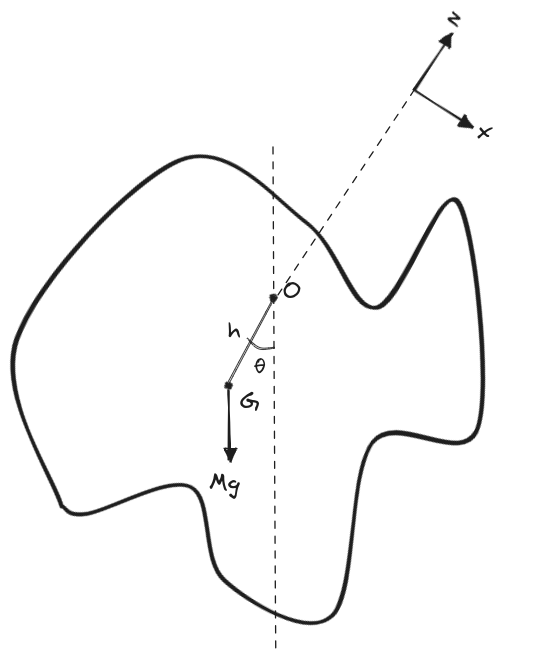
\includegraphics[scale=0.5]{ch11-10.png}
    \end{center}
    Where $G$ is the center of mass of the body and $\theta$
    is the angular displacement from the vertical line.

    We can treat this system as a planar rigid body hence it satisfies the
    Planar rigid body equations so the equations in the $x$ and $z$ direction
    give us 
    \begin{align*}
        M \ddot{\theta}h = Mg\sin\theta
        \quad\text{ and }\quad
        0 = Mg\cos\theta
    \end{align*}
    and from the momentum equation, we get that
    \begin{align*}
        I \ddot{\theta} = h Mg\sin\theta
    \end{align*}
    by replacing $Mg\sin\theta$ we get that
    \begin{align*}
        I\ddot{\theta} &= M \ddot{\theta}h^2\\
        h &= \frac{I}{Mh}
    \end{align*}
    Finally, we know that the period of small oscillations in a pendulum where
    $l$ is the length of the pendulum is given by
    \begin{align*}
        \tau = 2\pi \sqrt{\frac{l}{g}}
    \end{align*}
    Therefore, in this case, we get that
    \begin{align*}
        \tau = 2\pi \sqrt{\frac{I}{Mgh}}
    \end{align*}

    On the other hand, the period of small oscillations of a uniform rod of
    length $2a$, pivoted about a horizontal axis perpendicular to the rod and
    distance $b$ from its center can be computed from the above formula
    but first we need to compute the moment of inertial for the given system
    hence
    \begin{align*}
        I &= \int_{b-a}^{b+a} r^2 \frac{M}{2a} dr\\
        I &= \frac{M}{2a}\bigg[\frac{r^3}{3}\bigg]_{b-a}^{b+a}\\
        I &= \frac{M}{2a}\bigg[\frac{(b+a)^3}{3} - \frac{(b-a)^3}{3}\bigg]\\
        I &= M\bigg[\frac{a^2}{3} + b^2\bigg]
    \end{align*}
    Therefore the period of small oscillations is given by
    \begin{align*}
        \tau &= 2\pi \sqrt{\frac{M(a^2/3 + b^2)}{Mgb}}\\
        \tau &= 2\pi \sqrt{\frac{a^2 + 3b^2}{3gb}}
    \end{align*}
\end{proof}
\cleardoublepage
\begin{proof}{\textbf{11.11}}
    Let's consider the two stages of the system, shown below
    \begin{center}
        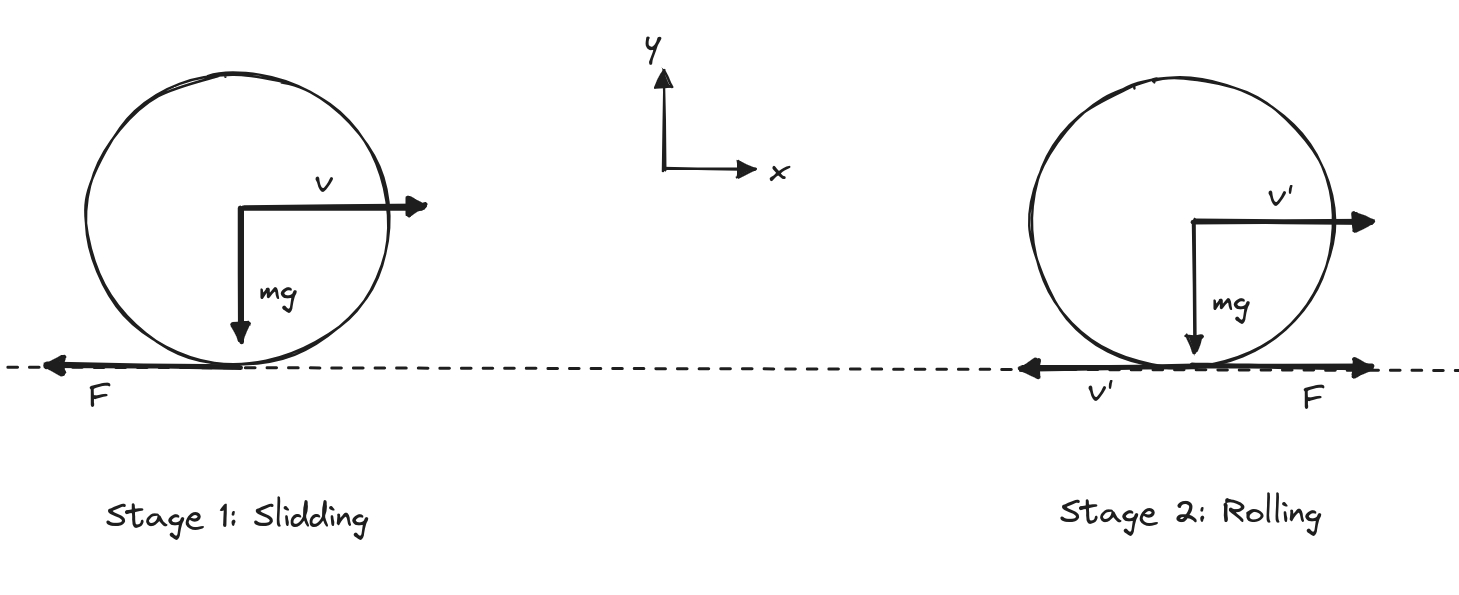
\includegraphics[scale=0.30]{ch11-11.png}
    \end{center}
    In stage 1 Newton's law in $x$ direction says that
    \begin{align*}
        m\frac{dv}{dt} = -F
    \end{align*}
    And in stage 2 the rotation equation says that
    \begin{align*}
        I \frac{d\omega}{dt} = rF
    \end{align*}
    By replacing the moment of inertia of the ball $I = 2/5 m r^2$ and
    the value of $F$ we got from the first equation we see that
    \begin{align*}
        \frac{2}{5}mr^2\frac{d\omega}{dt} &= -r m\frac{dv}{dt}\\
        \frac{2}{5}r\frac{d\omega}{dt} &= -\frac{dv}{dt}\\
        \frac{2}{5}r\frac{d\omega}{dt} + \frac{dv}{dt} &= 0
    \end{align*}
    Now we integrate with respect to $t$ then
    \begin{align*}
        \frac{2}{5}r\omega + v &= C
    \end{align*}
    Also, we know that initially $v = V$ and $\omega = 0$ so $C = V$ hence
    \begin{align*}
        \frac{2}{5}r\omega + v &= V
    \end{align*}
    If we now suppose that the ball rolls with speed $V'$ we know that
    $\omega = V'/r$ hence we get that
    \begin{align*}
        \frac{2}{5}V' + V' &= V\\
        V' &= \frac{5}{7}V
    \end{align*}
    
    Let us now compute the final kinetic energy of the ball assuming it is
    rolling (and maybe sliding) with velocity $V'$ hence
    \begin{align*}
        T' &= \frac{1}{2}mV'^2 +
        \frac{1}{2}\bigg(\frac{2}{5}m r^2\bigg)\bigg(\frac{V'^2}{r^2}\bigg)\\
        T' &= \frac{7}{10}mV'^2\\
        T' &= \frac{7}{10}m\bigg(\frac{25}{49}V^2\bigg)\\
        T' &= \frac{1}{2}m\frac{5}{7}V^2 = \frac{5}{7}T
    \end{align*}
    Where we used the value for $V'$ we computed earlier and we replaced
    $T = 1/2 ~mV^2$. Therefore the ball lost $2/7$ of it's initial kinetic
    energy.
\end{proof}
\cleardoublepage
\begin{proof}{\textbf{11.12}}
    Let's suppose the ball is rolling as shown below
    \begin{center}
        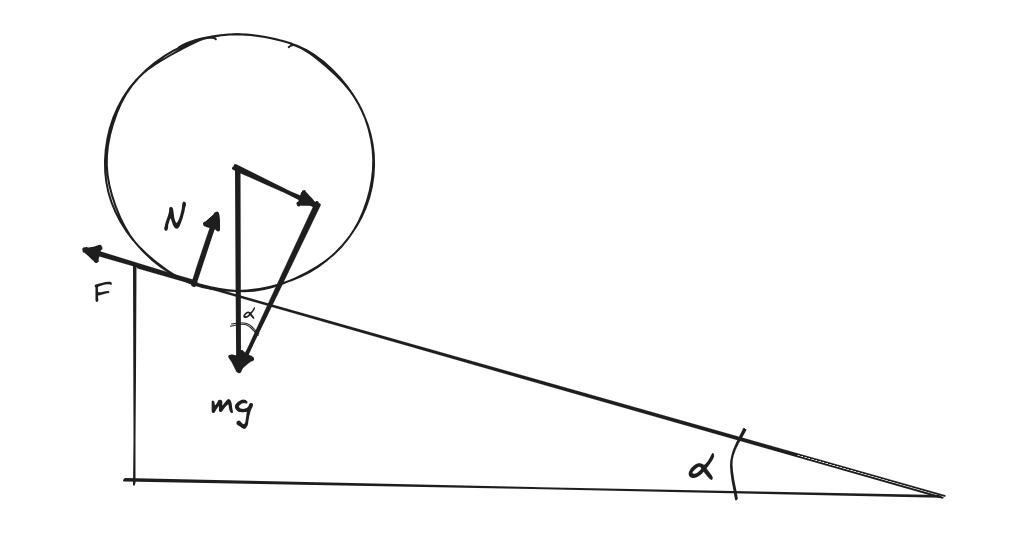
\includegraphics[scale=0.45]{ch11-12.png}
    \end{center}
    where $F$ is the friction force. Then the rolling equation where we are
    considering the positive rotation in the clockwise direction
    would be
    \begin{align*}
        I \frac{d\omega}{dt} &= rF\\
        \frac{2}{5}mr^2\frac{d\omega}{dt} &= r\mu mg\cos\alpha\\
        \frac{2}{5}r\frac{d\omega}{dt} &= g\mu \cos\alpha\\
        \frac{2}{5}\frac{dv}{dt} &= g\mu \cos\alpha
    \end{align*}
    We are replacing $F = \mu N = \mu (mg \cos\alpha)$,
    $d\omega/dt = 1/r\cdot dv/dt$ and $I = 2/5 mr^2$.

    From Newton's equation in the $x$ direction, we have the following
    \begin{align*}
        m \frac{dv}{dt} &= mg \sin\alpha - F\\
        \frac{dv}{dt} &= g(\sin\alpha - \mu \cos\alpha)
    \end{align*}
    Where we have the value for the acceleration in the case of a sliding ball
    since the equation is the same in a sliding situation.
    By replacing $dv/dt$ in the rolling equation we get that
    \begin{align*}
        \frac{2}{5}g(\sin\alpha - \mu \cos\alpha) &= g\mu \cos\alpha\\
        \frac{2}{5}\sin\alpha &= \frac{7}{5}\mu \cos\alpha\\   
        \frac{2}{7}\tan\alpha &= \mu   
    \end{align*}
    This implies that if $\mu < \frac{2}{7}\tan\alpha$ then rolling would be
    impossible and the ball would slide, and if $\mu \geq \frac{2}{7}\tan\alpha$
    then the ball would roll.

    Finally if we replace the value of $\mu$ in the last form of the rolling
    equation we get that
    \begin{align*}        
        \frac{dv}{dt} &= \frac{5}{2}g\bigg(\frac{2}{7}\tan\alpha\bigg)\cos\alpha\\
        \frac{dv}{dt} &= \frac{5}{7}g\sin\alpha
    \end{align*}
\end{proof}


\end{document}






















